% ------------------------------------------------------------------------
% Artigo 
% ------------------------------------------------------------------------

% Carga de parâmetros


\documentclass[
	% -- opções da classe memoir --
	article,			        % indica que é um artigo acadêmico
	11pt,				          % tamanho da fonte
	oneside,			        % para impressão apenas no verso. Oposto a twoside
	a4paper,			        % tamanho do papel. 
	english,			        % idioma adicional para hifenização
	brazil,				        % o último idioma é o principal do documento
	sumario=tradicional
]{abntex2}\usepackage[]{graphicx}\usepackage[]{color}
%% maxwidth is the original width if it is less than linewidth
%% otherwise use linewidth (to make sure the graphics do not exceed the margin)
\makeatletter
\def\maxwidth{ %
  \ifdim\Gin@nat@width>\linewidth
    \linewidth
  \else
    \Gin@nat@width
  \fi
}
\makeatother

\definecolor{fgcolor}{rgb}{0.345, 0.345, 0.345}
\newcommand{\hlnum}[1]{\textcolor[rgb]{0.686,0.059,0.569}{#1}}%
\newcommand{\hlstr}[1]{\textcolor[rgb]{0.192,0.494,0.8}{#1}}%
\newcommand{\hlcom}[1]{\textcolor[rgb]{0.678,0.584,0.686}{\textit{#1}}}%
\newcommand{\hlopt}[1]{\textcolor[rgb]{0,0,0}{#1}}%
\newcommand{\hlstd}[1]{\textcolor[rgb]{0.345,0.345,0.345}{#1}}%
\newcommand{\hlkwa}[1]{\textcolor[rgb]{0.161,0.373,0.58}{\textbf{#1}}}%
\newcommand{\hlkwb}[1]{\textcolor[rgb]{0.69,0.353,0.396}{#1}}%
\newcommand{\hlkwc}[1]{\textcolor[rgb]{0.333,0.667,0.333}{#1}}%
\newcommand{\hlkwd}[1]{\textcolor[rgb]{0.737,0.353,0.396}{\textbf{#1}}}%

\usepackage{framed}
\makeatletter
\newenvironment{kframe}{%
 \def\at@end@of@kframe{}%
 \ifinner\ifhmode%
  \def\at@end@of@kframe{\end{minipage}}%
  \begin{minipage}{\columnwidth}%
 \fi\fi%
 \def\FrameCommand##1{\hskip\@totalleftmargin \hskip-\fboxsep
 \colorbox{shadecolor}{##1}\hskip-\fboxsep
     % There is no \\@totalrightmargin, so:
     \hskip-\linewidth \hskip-\@totalleftmargin \hskip\columnwidth}%
 \MakeFramed {\advance\hsize-\width
   \@totalleftmargin\z@ \linewidth\hsize
   \@setminipage}}%
 {\par\unskip\endMakeFramed%
 \at@end@of@kframe}
\makeatother

\definecolor{shadecolor}{rgb}{.97, .97, .97}
\definecolor{messagecolor}{rgb}{0, 0, 0}
\definecolor{warningcolor}{rgb}{1, 0, 1}
\definecolor{errorcolor}{rgb}{1, 0, 0}
\newenvironment{knitrout}{}{} % an empty environment to be redefined in TeX

\usepackage{alltt}


% ---
% PACOTES
% ---

% ---
% Pacotes fundamentais 
% ---
\usepackage{lmodern}			    % Usa a fonte Latin Modern
\usepackage[T1]{fontenc}		  % Selecao de codigos de fonte.
\usepackage[utf8]{inputenc}		% Codificacao do documento (conversão automática dos acentos)
\usepackage{indentfirst}   		% Indenta o primeiro parágrafo de cada seção.
\usepackage{nomencl}  		  	% Lista de simbolos
\usepackage{color}				    % Controle das cores
\usepackage{graphicx}			    % Inclusão de gráficos
\usepackage{microtype} 			  % para melhorias de justificação
\usepackage[alf,abnt-etal-cite=1]{abntex2cite}
\usepackage{amsmath}
\usepackage{amssymb}
\usepackage{amsfonts}


%\usepackage{draftwatermark}

% ---
		
% ---
% Pacotes adicionais, usados apenas no âmbito do Modelo Canônico do abnteX2
% ---

% ---
		
% ---
% Pacotes de citações
% ---
\usepackage[brazilian,hyperpageref]{backref}	 % Paginas com as citações na bibl
\usepackage{everypage}
\AddEverypageHook{DRAFT VERSION}

% ---

% ---
% Configurações do pacote backref
% Usado sem a opção hyperpageref de backref
\renewcommand{\backrefpagesname}{Citado na(s) página(s):~}
% Texto padrão antes do número das páginas
\renewcommand{\backref}{}

% ---

% ---
% Informações de dados para CAPA e FOLHA DE ROSTO
% ---
\titulo{Jogos cooperativos na\\ gestão da cadeia de suprimentos}

\author{João B. G. Brito, \emph{Esp.}   \\   
    \href{mailto:jbgb@uol.com.br}{jbgb@uol.com.br} 
  \and {Michel J. Anzanello, \emph{Phd}} \\
    \href{mailto:michel.anzanello@gmail.com}{michel.anzanello@gmail.com}
}

\date{\today}

\instituicao{
    Escola de Engenharia de Produção \\
    Universidade Federal do Rio Grande do Sul -- UFRGS \\
  Logística e Gestão da Cadeia de Suprimentos - 2015
}

\local{Av. Osvaldo Aranha, 99 – 5º andar, CEP: 90035-190, Porto Alegre/RS}

% ---
% Configurações de aparência do PDF final

% alterando o aspecto da cor azul
\definecolor{blue}{RGB}{41,5,195}

% informações do PDF
\makeatletter
\hypersetup{
     	%pagebackref=true,
		pdftitle={\@title}, 
		pdfauthor={\@author},
    	pdfsubject={\@title},
	    pdfcreator={\@author},
  	pdfkeywords={Teoria dos jogos cooperativos}
                {Gestão da cadeia de suprimentos}
                {Shapley value}
                {Per capita nucleolus}
                {Nucleolus}, 
   	 colorlinks=true,       	  % false: boxed links; true: colored links
     	linkcolor=blue,          	% color of internal links
    	citecolor=blue,        		% color of links to bibliography
    	filecolor=magenta,      	% color of file links
		urlcolor=blue,
		bookmarksdepth=4
}
\makeatother
% --- 

% compila o indice
% ---
\makeindex
% ---

% ---
% Altera as margens padrões
% ---
\setlrmarginsandblock{3cm}{3cm}{*}
\setulmarginsandblock{3cm}{3cm}{*}
\checkandfixthelayout
% ---

% --- 
% Espaçamentos entre linhas e parágrafos 
% --- 

% O tamanho do parágrafo é dado por:
\setlength{\parindent}{1.3cm}

% Controle do espaçamento entre um parágrafo e outro:
\setlength{\parskip}{0.2cm}  % tente também \onelineskip

% Espaçamento simples
\SingleSpacing

% ----
% Início do documento
% ----
\IfFileExists{upquote.sty}{\usepackage{upquote}}{}
\begin{document}

% Seleciona o idioma do documento (conforme pacotes do babel)
%\selectlanguage{english}
\selectlanguage{brazil}

% Retira espaço extra obsoleto entre as frases.
\frenchspacing 

% ----------------------------------------------------------
% ELEMENTOS PRÉ-TEXTUAIS
% ----------------------------------------------------------

%---
%
% Se desejar escrever o artigo em duas colunas, descomente a linha abaixo
% e a linha com o texto ``FIM DE ARTIGO EM DUAS COLUNAS''.
%
%---
% página de titulo
\maketitle

% resumo em português
\begin{resumoumacoluna}
% Contextualização: 
% Gap:
% Proposta: 
% Metodologia
% Resultados
% Conclusão 
No ambiente de uma gestão cadeia de suprimentos (GCS) as decisões de cada organização tendem a refletir nos seus elos. A análise destas interações é importante para avaliar a colaboração entre seus membros, sugerir acordos e buscar o equilíbrio mais rentável. Para explorar problemas desta espécie propomos o emprego da teoria dos jogos cooperativos (TJC) com um algorítmo que maximiza a satisfação dos insatisfeitos (\emph{nucleolus}) e outro que pondera a participação nos custos de cada parceiro (\emph{Shapley value}). Para execução, iniciamos com a apreciação dos conceitos da TJC relacionando com a GCS, para então explorar o raciocínio de cada lógica e discutir a comparação deles. Como resultados, encontramos \texttt{(adicionar os resultados)}. Concluímos que o \emph{nucleolus} e \emph{Shapley value} tem potencial de instrumentar apoio na definição de diretrizes da GCS pois seu emprego oferece recursos para racionalizar o potencial dos relacionamentos, estratégias conflitantes e colaborativas.

 \vspace{\onelineskip}
 
 \noindent
 \textbf{Palavras-chave}: Agentes da cadeia de suprimentos. Otimiza\c{c}{\~a}o. Teoria dos Jogos. Shapley value. Nucleolus.
\end{resumoumacoluna}

% ---

% ----------------------------------------------------------
% ELEMENTOS TEXTUAIS
% ----------------------------------------------------------
\textual

% \twocolumn[    		    
% ]      		% FIM DE ARTIGO EM DUAS COLUNAS
% ----------------------------------------------------------
% Introdução
% ----------------------------------------------------------
\section*{Introdução}
\addcontentsline{toc}{section}{Introdução}

\texttt{\color{red}...criar seção...}

  \begin{itemize}
    \item Theory of games and economic behavior \cite{Neumann.1947}
    \item Social choice and individual values \cite{Figueiredo.1994}
    \item Teoria dos Jogos Cooperativos: Conceitos Fundamentais \cite{Moreira.2002}
    \item Teoria Dos Jogos \cite{Fiani.2006}
    \item Bayesian learning in negotiation \cite{Zeng.1998}
    \item Teoria dos Jogos \cite{Tavares.2009}
    \item Teoria dos Jogos \cite{Bierman.2010}
    \item Coopera\c{c}{\~a}o e Conflito \cite{Fiani.2011}
    \item Teoria dos Jogos: Crenas, Desejos e Escolhas \cite{Paula.2014}
    \item A Way to Play Claims Problems \cite{Gimenez.2014}
    \item Teoria dos Jogos \cite{Fiani.2015}
    \item Entrevista com Bruce Bueno de Mesquita \cite{Mesquita.2012}
  \end{itemize}

% ----------------------------------------------------------
% Seção conexão entre teoria dos jogos até cooperativos
% ----------------------------------------------------------
\section{Teoria dos jogos cooperativos}

A chave da cooperação entre empresas está em conseguir a unidade de motivação pelo alinhamento de incentivos \cite{Cao.2012}. Uma cadeia de suprimentos é beneficiada pela colaboração entre seus membros, que pode ocorrer pelo compartilhamento de informações, conhecimentos, custos, riscos e recompensas. Mesmo que as organizações constituam unidades autônomas, temos uma sequência ou rede de relações interdependentes que pode promover alianças estratégicas \cite{Chen.2004}. Em geral, a cooperação vem ganhando cada vez mais importância, principalmente em redes de alta complexidade \cite{Drechsel.2010} onde as decisões de cadados membros (agentes) afeta nas decisões dos demais e o acordo entre os agentes é a base da cooperação \cite{Young.1994}.

\begin{equation}
  \label{eq:conceitoTJC}
  \left \{ 
    \emph{x} \in \Re^{\emph{n}} \mid f\left ( x,S \right ) \leq c\left ( S \right ), \forall \emph{S} \subseteq \emph{N}
  \right\}
\end{equation}

\texttt{\color{red}...seguem referências para seção...}

  \begin{itemize}
    \item Linearity of unrestrictedly transferable utilities \cite{Aumann.1960}
    \item Introduction to the Theory of Cooperative Games \cite{Peleg.2007}
    \item Game Theory Cooperative Games with Transferable Utility \cite{Peters.2008}
  \end{itemize}
  
% ----------------------------------------------------------
% Seção conexão entre teoria dos jogos e cadeia de suprimentos
% ----------------------------------------------------------
\section{Gerenciamento da Cadeia de suprimentos}

Estudos sobre a aplicação da teoria dos jogos cooperativos no gerencimento da cadeia de suprimentos abordam como principal questão o gerenciamento harmonioso das decisões entre os elos da cadeia \cite{Dobos.2010a}. O pressuposto está na existência de uma estrutura comum entre os agentes de uma cadeia e que o ganho ou custo seja compartilhado seguindo critérios de distribuição (axiomas)\cite{Bezerra.2009}.

  \begin{itemize}
    \item Aplicação de Teoria de Jogos à Alocação de Capacidade Firme em um Sistema Térmico \cite{Ayala.2008}
    \item Value Solutions in Cooperative Games \cite{Mccain.2013} 
    \item Cooperative Games, Solutions and Applications \cite{Driessen.2013}
    \item A Teoria dos Jogos Aplicada ao Processo Penal \cite{Rosa.2014}
    \item Towards a theory of supply chain management: the constructs and measurements \cite{Chen.2004}
    \item Game Theory in Supply Chain Analysis \cite{Cachon.2004}
    \item Supply Chain Games: Operations Management and Risk Valuation \cite{kogan.2007}
    \item Cooperation: Game-Theoretic Approaches \cite{Hart.2012}
    \item Quantitative Methods in Supply Chain Management: Models and Algorithms \cite{Christou.2012}
    \item Cooperation in an HMMS-type supply chain: A management application of cooperative game theory \cite{Dobos.2010b}
  \end{itemize}

% ----------------------------------------------------------
% Estudo de caso
% ----------------------------------------------------------
\section{Estudo de caso}

  \texttt{\color{red}...linguagem e pacotes da seção...}
  \begin{itemize}
    \item R: A Language and Environment for Statistical Computing \cite{R.2016}
    \item ggmap: Spatial Visualization with ggplot2 \cite{Kahle.2013}
  \end{itemize}

\begin{knitrout}
\definecolor{shadecolor}{rgb}{0.969, 0.969, 0.969}\color{fgcolor}\begin{figure}[!h]

{\centering 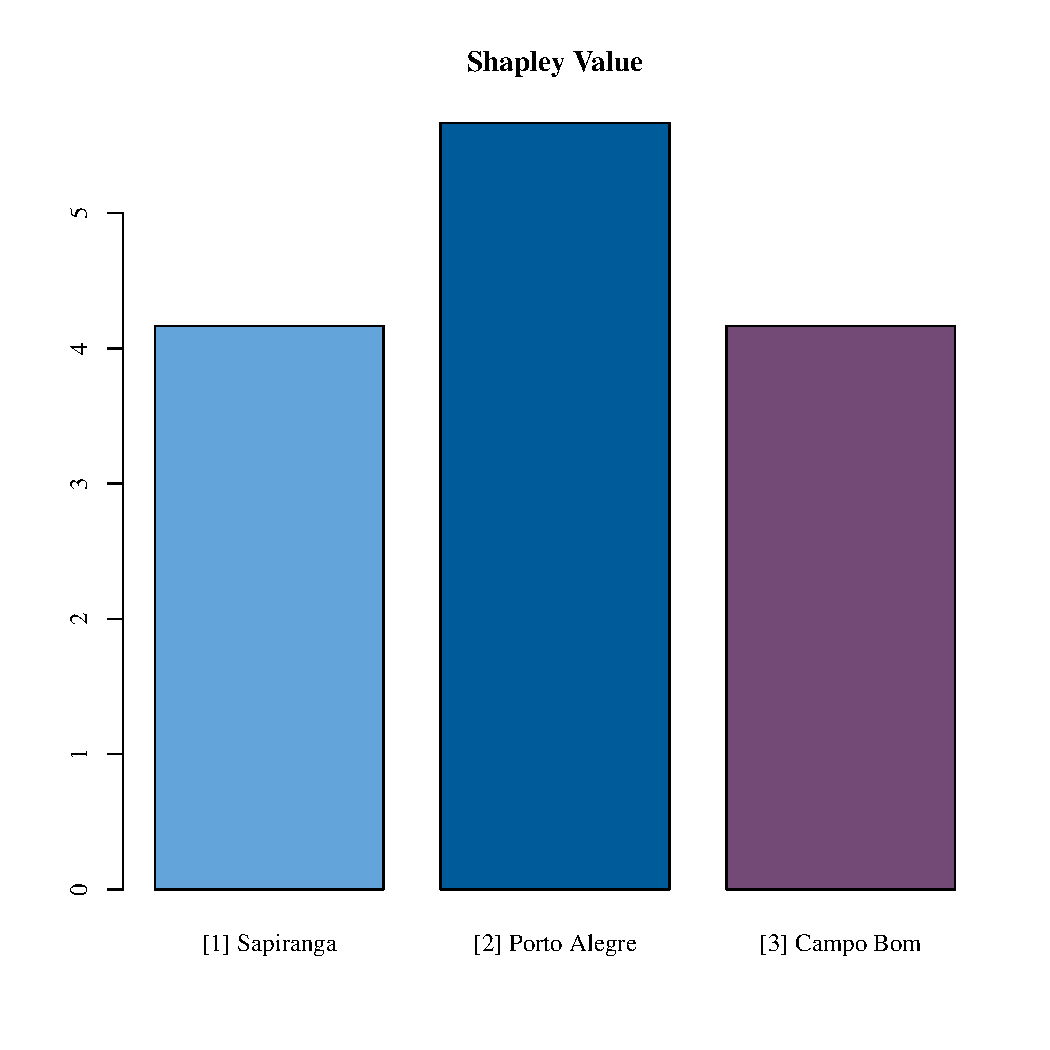
\includegraphics[width=\maxwidth]{figure/unnamed-chunk-2-1} 

}

\caption[Itinerários]{Itinerários}\label{fig:unnamed-chunk-2}
\end{figure}


\end{knitrout}

\begin{table}[!h]
  \centering
  \caption{Tabela de combinações de agentes e custo}
  \label{Tab1}
  \begin{tabular}{@{}cccccccccc@{}}
  \toprule
    $S$    & $\emptyset$ & $\{1\}$ & $\{2\}$ & $\{3\}$ & $\{1,2\}$ & $\{1,3\}$ & $\{2,3\}$ &     $\{1,2,3\}$ & $N$  \\ \midrule
    $v(S)$ & $0$         & $5$     & $8$     & $5$     & $10$      & $10$      & $10$      &     $14$        & $14$ \\ \bottomrule
  \end{tabular}
\end{table}

% ----------------------------------------------------------
% Shapley value
% ----------------------------------------------------------
\section{\emph{Shapley value}}

\subsection{\emph{Conceito}}

Shapley axiomas para $\varphi(v)$
\begin{enumerate}
  \item Eficiência: $\sum_{i \in N} \varphi_i(v) - v(N)$. Toda a alocação 
  \item Simetria: Se $i$ e $j$ são tal que $v(S \cup \{i\}) = v(S \cup \{j\})$ para cada coalisão $S$ não contenha $i$ e $j$, então $\varphi_i (v) = \varphi_j (v)$
  \item 
\end{enumerate}

Sendo $\forall$ $S \neq \emptyset$ e $S \subset N$

\begin{equation}
  \label{eq:shaVal}
  \varphi _{i} = \sum_{S \subset N} \frac{(|s| - 1)!(n - |s|)!}{n!}[v(S)-v(S - i)]
\end{equation}

Consideramos 

Para $i = 1$.

\begin{subequations}
  \tiny
  \begin{equation}
   \label{eq:shaValX1a}
    x_{[1]} = \frac{0!2!}{3!}(c(\{1\}) - c(\emptyset)) +
              \frac{1!1!}{3!}(c(\{1,2\}) - c(\{2\}) +
              \frac{1!1!}{3!}(c(\{1,3\}) - c(\{3\}) +
              \frac{2!0!}{3!}(c(\{1,2,3\}) - c(\{2,3\}) 
  \end{equation}

  $\therefore$

  \begin{equation}
   \label{eq:shaValX1b}
    x_{[1]} = \frac{2}{6}(c(\{5 - 0\}) +
              \frac{1}{6}(c(\{10 - 8\}) +
              \frac{1}{6}(c(\{10 - 5\}) +
              \frac{2}{6}(c(\{14 - 10\})
  \end{equation}

  $\therefore$

  \begin{equation}
   \label{eq:shaValX1c}
    x_{[1]} = \frac{25}{6} \cong 4,1667
   \end{equation}
\end{subequations}                  

Para $i = 2$.

\begin{subequations}
  \tiny
  \begin{equation}
   \label{eq:shaValX2a}
    x_{[2]} = \frac{0!2!}{3!}(c(\{2\}) - c(\emptyset)) +
              \frac{1!1!}{3!}(c(\{1,2\}) - c(\{1\}) +
              \frac{1!1!}{3!}(c(\{2,3\}) - c(\{3\}) +
              \frac{2!0!}{3!}(c(\{1,2,3\}) - c(\{1,3\}) 
  \end{equation}

  $\therefore$

  \begin{equation}
   \label{eq:shaValX2b}
    x_{[2]} = \frac{2}{6}(c(\{8 - 0\}) +
              \frac{1}{6}(c(\{10 - 5\}) +
              \frac{1}{6}(c(\{10 - 5\}) +
              \frac{2}{6}(c(\{14 - 10\})
  \end{equation}

  $\therefore$

  \begin{equation}
   \label{eq:shaValX2c}
    x_{[2]} = \frac{34}{6} \cong 5,6667
   \end{equation}
\end{subequations}                  

Para $i = 3$.

\begin{subequations}
  \tiny
  \begin{equation}
   \label{eq:shaValX3a}
    x_{[3]} = \frac{0!2!}{3!}(c(\{3\}) - c(\emptyset)) +
              \frac{1!1!}{3!}(c(\{1,3\}) - c(\{1\}) +
              \frac{1!1!}{3!}(c(\{2,3\}) - c(\{2\}) +
              \frac{2!0!}{3!}(c(\{1,2,3\}) - c(\{1,2\}) 
  \end{equation}
  
  $\therefore$
  
  \begin{equation}
   \label{eq:shaValX3b}
    x_{[3]} = \frac{2}{6}(c(\{5 - 0\}) +
              \frac{1}{6}(c(\{10 - 5\}) +
              \frac{1}{6}(c(\{10 - 8\}) +
              \frac{2}{6}(c(\{14 - 10\})
  \end{equation}

  $\therefore$

  \begin{equation}
   \label{eq:shaValX3c}
    x_{[3]} = \frac{25}{6} \cong 4,1667
   \end{equation}
\end{subequations}                  

A solução para o vetor $x$ é:

\begin{equation}
 \label{eq:shaValXSol}
  x = \left ( 
        \frac{25}{6}; \
        \frac{34}{6}; \
        \frac{25}{6}
      \right ) 
\end{equation}

$\therefore$

\begin{equation}
 \label{eq:shaValXSolApx}
  x \cong \left (4,1667; 5,6667; 4,1667 \right ) 
\end{equation}

Onde:

\begin{equation}
 \label{eq:shaValXProva}
  x = \left ( 
        \frac{25}{6} +
        \frac{34}{6} +
        \frac{25}{6}
      \right )
\end{equation}

$\because$

\begin{equation}
 \label{eq:shaValXPorque}
 \sum_{i = 1}^{3}x_i = 14 = c(N)
\end{equation}

\texttt{\color{red}...seguem referências para seção...}
  
  \begin{itemize}
    \item Aircraft Landing Fees: A Game Theory Approach \cite{Littlechild.1977}
    \item The Shapley value: essays in honor of Lloyd S. Shapley \cite{Alvin.1988}
    \item Lloyd Shapley's Matching and Game Theory \cite{Serrano.2013}
    \item Cooperative Game Theory and Applications: Cooperative Games Arising from Combinatorial Optimization Problems \cite{Curiel.2013}
    \item On axiomatizations of the Shapley value for assignment games \cite{Brink.2015}
  \end{itemize}

\subsection{Código em R}

  \texttt{\color{red}...linguagem e pacotes da seção...}

  \begin{itemize}
    \item R: A Language and Environment for Statistical Computing \cite{R.2016}
    \item scales: Scale Functions for Visualization \cite{Wickham.2015}
    \item ggplot2: Elegant Graphics for Data Analysis \cite{Wickham.2009}
  \end{itemize}

\begin{knitrout}
\definecolor{shadecolor}{rgb}{0.949, 0.949, 0.949}\color{fgcolor}\begin{kframe}
\begin{verbatim}
# Define os custos de coalisoes
coalisoesAgentes <- c(5, 8, 5, 10, 10, 10, 14)

# Nomes dos agentes/jogadores
nomesAgentes <- c("[1] Sapiranga","[2] Porto Alegre","[3] Campo Bom")

# Define jogo com tres jogadores/agentes
definicaoJogo   <- DefineGame(3, coalisoesAgentes)

# Demonstra as coalisoes e res  pectivos custos
summary(definicaoJogo)

# Calcula o Shapley Value
shapleyValue <- ShapleyValue(x = definicaoJogo, 
                             Names = nomesAgentes)
# Guarda o resultado
valorShapley <- summary(shapleyValue)
\end{verbatim}
\end{kframe}
\end{knitrout}

\begin{knitrout}
\definecolor{shadecolor}{rgb}{0.969, 0.969, 0.969}\color{fgcolor}\begin{figure}[h]

{\centering 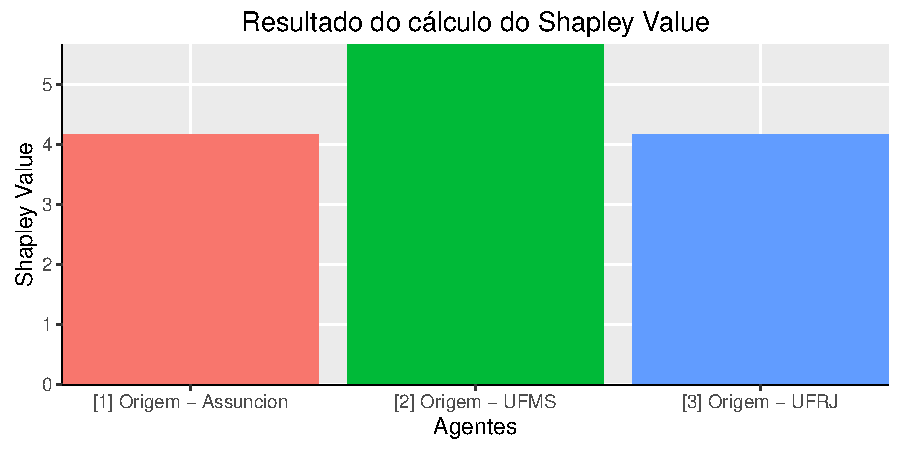
\includegraphics[width=\maxwidth]{figure/unnamed-chunk-4-1} 

}

\caption[Cálculo do valor de Shapley]{Cálculo do valor de Shapley}\label{fig:unnamed-chunk-4}
\end{figure}


\end{knitrout}

\section{\emph{Nucleolus}}

\texttt{\color{red}...seguem referências para seção...}
  
  \begin{itemize}
    \item The Nucleolus of a Characteristic Function Game \cite{Schmeidler.1969}
    \item Geometric Properties of the Kernel, Nucleolus, and Related Solution Concepts \cite{Maschler.1979}
    \item Game theoretic analysis of a bankruptcy problem from the Talmud \cite{Aumann.1985}
    \item Game Theory (An Introduction) \cite[p. 219--307]{Barron.2007}
    \item Collective Rationality: Equilibrium in Cooperative Games \cite{Weirich.2009}
    \item Prática na Teoria. Aplicações da Teoria dos Jogos e da Evolução aos Negócios \cite{Marinho.2011}
    \item Common mistakes in computing the nucleolus \cite{Guajardo.2015}
    \item O Dilema do Prisioneiro desde Hegel até Lacan: Tomo 1 \cite{Faveret.2015}
  \end{itemize}

\section{Análise comparativa}

\texttt{\color{red}...seguem referências para seção...}

  \begin{itemize}
    \item A cooperative game in search theory \citet{Hohzaki.2009}

  \end{itemize}

% ---
% Finaliza a parte no bookmark do PDF, para que se inicie o bookmark na raiz
% ---
\bookmarksetup{startatroot}% 
% ---

% ---
% Conclusão
% ---
\section*{Conclusão}

% ----------------------------------------------------------
% ELEMENTOS PÓS-TEXTUAIS
% ----------------------------------------------------------
\postextual

% ---
% Título e resumo em língua estrangeira
% ---

% \twocolumn[    		% INICIO DE ARTIGO EM DUAS COLUNAS

% ]  				        % FIM DE ARTIGO EM DUAS COLUNAS
% ---

% ----------------------------------------------------------
% Referências bibliográficas
% ----------------------------------------------------------
\bibliography{references}

\end{document}


% ----------------------------------------------------------
% Glossário
% ----------------------------------------------------------
%
% Há diversas soluções prontas para glossário em LaTeX. 
% Consulte o manual do abnTeX2 para obter sugestões.
%
%\glossary

% ----------------------------------------------------------
% Apêndices
% ----------------------------------------------------------

% ---
% Inicia os apêndices
% ---
\begin{apendicesenv}

% ----------------------------------------------------------
\chapter{}
% ----------------------------------------------------------

\end{apendicesenv}
% ---

% ----------------------------------------------------------
% Anexos
% ----------------------------------------------------------
\cftinserthook{toc}{AAA}
% ---
% Inicia os anexos
% ---
%\anexos
\begin{anexosenv}

% ---
\chapter{}
% ---

\end{anexosenv}
